
\documentclass{cmc}

\begin{document}

\pagestyle{fancy}
\lhead{\textit{\textbf{Computational Motor Control, Spring 2018} \\
    Python exercise, Lab 7, GRADED}} \rhead{Student \\ Names}

\section*{Student names: \ldots (please update)}

\textit{Instructions: Update this file (or recreate a similar one,
  e.g.\ in Word) to prepare your answers to the questions. Feel free
  to add text, equations and figures as needed. Hand-written notes,
  e.g.\ for the development of equations, can also be included e.g.\
  as pictures (from your cell phone or from a scanner).
  \textbf{\corr{This lab is graded.}} and needs to be submitted before
  the \textbf{\corr{Deadline : 03-06-2018
      Midnight}}.\\
  \textbf{\corr{You only need to submit one final report for all of
      the following exercises combined henceforth.}}\\ Please submit
  both the source file (*.doc/*.tex) and a pdf of your document, as
  well as all the used and updated Python functions in a single zipped
  file called \corr{final\_report\_name1\_name2\_name3.zip} where
  name\# are the team member’s last names.  \corr{Please submit only
    one report per team!}}
\\

\subsection*{Mouse Model}
\label{sec:mouse-model}
In this exercise you will be working with the hind-limb
musculoskeletal model of the mouse. The goal of the following
exercises will be to develop and understand how reflexes alone can
generate locomotion behavior. In order to do this we use the work of
[1] to develop the reflex model. Here you will integrate the concepts
learnt during the course to produce locomotion behavior.

\subsection*{Model Description}
\label{sec:model-description}

For the purpose of these exercises you will be using the mouse model
show in figure \ref{fig:mouse}. Since the main focus of the exercises
is to study hind limb locomotion, the fore limbs of the mouse are
rigidly fixed in a default position and only aid the mouse in balance
and stability during locomotion. The spine, head and pelvis are also
fixed a default position during locomotion. The hind limbs are the
most important entities of the following exercises.

\begin{figure}[H]
  \centering
  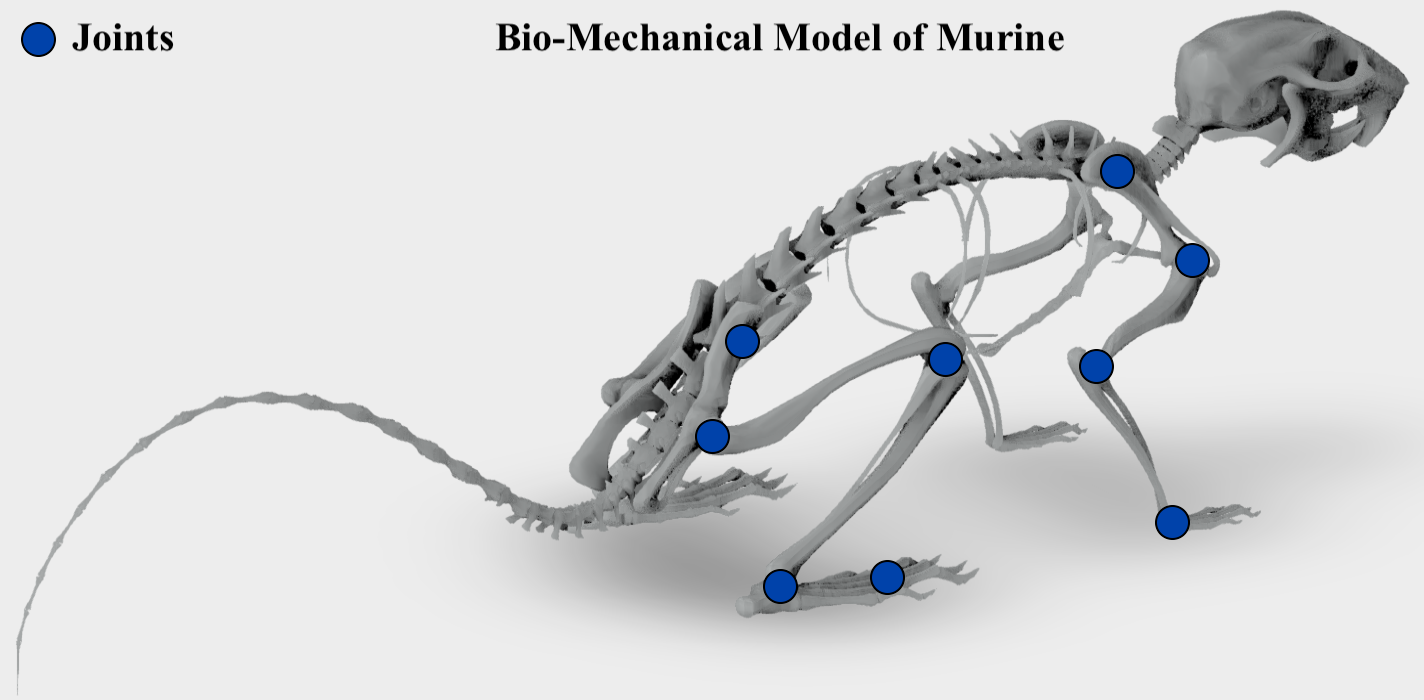
\includegraphics[width=\textwidth]{figures/mouse_model.png}
  \caption{Mouse Model used in the exercises}
  \label{fig:mouse}
\end{figure}

Figure \ref{fig:hind_limb_joints_muscles} shows the joints and muscles
considered for each of the two hind limbs in the mouse model.

\subsubsection*{Joints}
\label{sec:joints}

Each hind limb consists of four revolute joints,

\begin{itemize}
\item Hip
\item Knee
\item Ankle
\item MTP
\end{itemize}

Out of the four joints listed above, every joint actuated by at least
one pair of antagonist muscle pairs expect for the MTP joint. MTP
joint is passive and contains only a spring-damper to allow the joint
to return to its initial position.  To simplify the model, simpler
bounding box shapes are used to wrap the complex bone meshes.

\subsubsection*{Muscles}
\label{sec:muscles}

Each joint mentioned above is actuated by at least one pair of
antagonist muscles so that the joint can have the complete range of
motion. The set of muscles in each hind limb are show in figure
\ref{fig:hind_limb_muscles}. A mono-articular muscle applies a joint
torque on only one joint and a bi-articular muscle spans over two
joints and applies a torque on both.

To summarize, table \ref{tab:muscles} shows the list of muscles chosen
for simulation along with the joints about which they act and their
function on these joints in the hind limb.
	
	\begin{table}[H]
          \centering
          \begin{tabular}{|c|c|c|c|c|c|}
            \hline
            \textbf{Muscle}       & \textbf{Abbreviation} & \textbf{Type } & \textbf{Hip} & \textbf{Knee} & \textbf{Ankle} \\ \hline
            Psoas Major           & PMA                   & Mono-articular & Flexion      & -             & -              \\ \hline
            Caudofemoralis        & CF                    & Mono-articular & Extension    & -             & -              \\ \hline
            Semimembranosus       & SM                    & Bi-articular   & Extension    & Flexion       & -              \\ \hline
            Popliteus             & POP                   & Mono-articular & -            & Flexion       & -              \\ \hline
            Rectus Femoris        & RF                    & Mono-articular & -            & Extension     & -              \\ \hline
            Tibialis Anterior     & TA                    & Mono-articular & -            & -             & Dorsiflexion   \\ \hline
            Soleus                & SOL                   & Mono-articular & -            & -             & Plantarflexion \\ \hline
            Lateral Gastrocnemous & LG                    & Bi-articular   & -            & Flexion       & Plantarflexion \\ \hline
          \end{tabular}
          \caption{Summary of mouse hind limb muscles used in
            simulation}
          \label{tab:muscles}
	\end{table}

\begin{figure}[H]
  \centering
  \begin{subfigure}[b]{0.49\textwidth}
    { \centering
      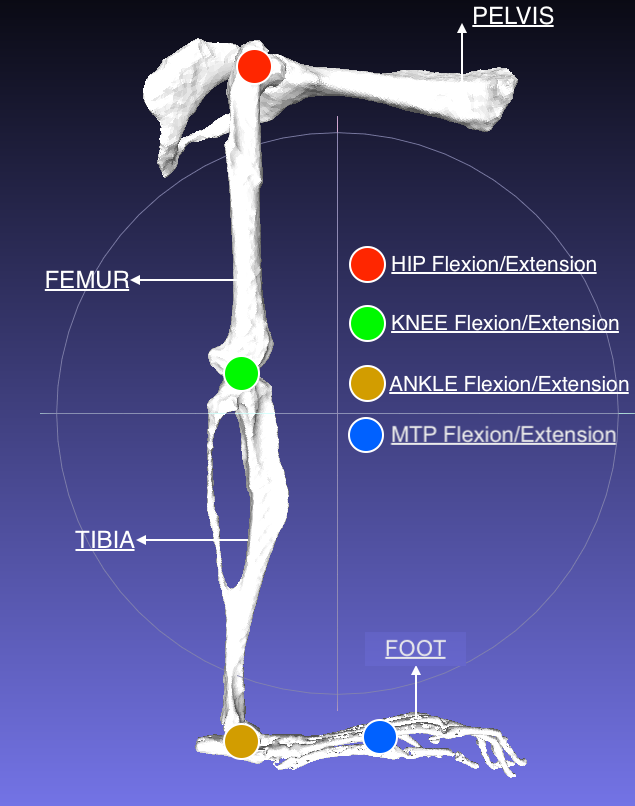
\includegraphics[width=\textwidth]{figures/HindLimbJoints.png} }
    \caption{Mouse hind limb joints}
    \label{fig:hind_limb_joints}
  \end{subfigure}
  \begin{subfigure}[b]{0.49\textwidth}
    { \centering
      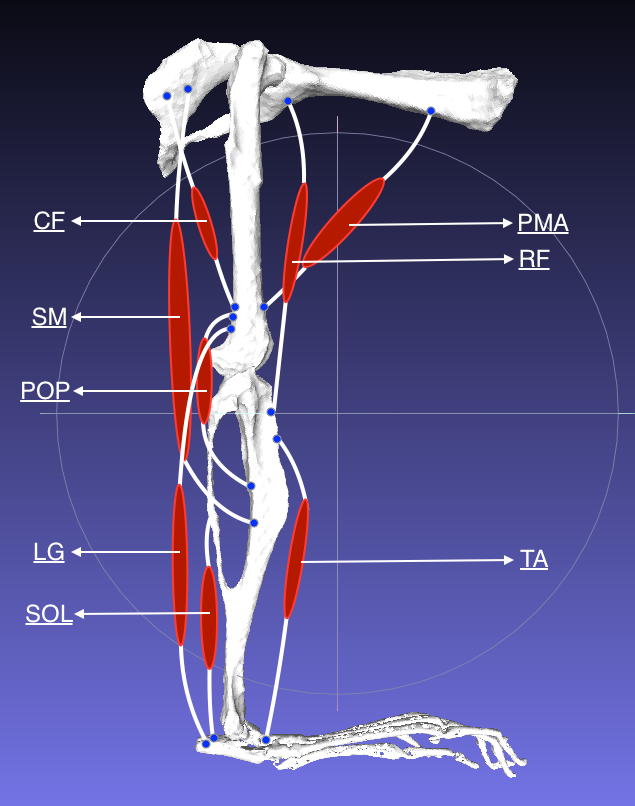
\includegraphics[width=\textwidth]{figures/HindLimbMuscles.png}
    }
    \caption{Mouse hind limb muscles}
    \label{fig:hind_limb_muscles}
  \end{subfigure}
  \caption{Mouse hind limb joints and muscles description}
  \label{fig:hind_limb_joints_muscles}
\end{figure}

\subsubsection*{Model Parameters}
\label{sec:model-parameters}

The model consists of two sets of important parameters. One, the
skeletal parameters and second the muscle parameters. All parameters
for joints and muscles are described in
\corr{musculoskeletal::mouse.json} file.

\textbf{Skeletal Parameters:}
\begin{itemize}
\item $mass$ : Mass of the bone [$kg$]
\item $size$ : Bone length, width and breadth [$m$]. Mesh bounding box
  defines these elements in the simulation.
\item $inertia$ : Moment of inertia [$kg-m^2$]
\item $center of mass$ : Center of mass of each segment [$m$]
\end{itemize}

\textit{NOTE : Refer to section Model Scaling for units used in the
  simulation}

The properties of each skeletal segment can be found in the world
editor in Webots .wbt file.

The muscle parameters are defined in a parameter .json file. The json
file contains the following parameters for each muscle and joint
present in the hind limb.

\textbf{Muscle Parameters:}
\begin{itemize}
\item $l_{opt}$ : Muscle optimal fiber length [$m$]
\item $l_{slack}$ : Muscle tendon slack length [$m$]
\item $theta\_ref(\theta_{ref})$ : Joint angle at which muscle is at
  its resting length [$deg$]
\item $theta\_max (\theta_{max})$ : Joint angle at which maximal
  muscle moment arm [$deg$]
\item $pennation$ : Fiber angle [$deg$]
\item $r_0$ : Maximum muscle moment arm [$m$]
\item $f_{max}$ : Maximum muscle force [$N$]
\item $v_{max}$ : Maximum muscle velocity [$l_{opt}/s$]
\item $joint\_attach$ : Joint to which the muscle exerts a moment
\item $direction$ : '\textit{clockwise} / \textit{cclockwise}' :
  Direction of muscle moment
\item $muscle\_type$ : '\textit{mono}' if muscle spans across only one
  joint. '\textit{bi}' if muscle spans across two joints. If muscle is
  bi-articular then $r_{02}$, $theta\_ref2$, $theta\_ref2$,
  $joint\_attach2$ and $direction2$ must be additionally defined for
  the second joint.
\end{itemize}

\textbf{Joint Parameters:}
\begin{itemize}
\item $joint\_type$ : 'CONSTANT' - Muscle moment arm computation type
\item $theta\_min$ : Minimum joint angle [$deg$]
\item $theta\_max$ : Maximum joint angle [$deg$]
\item $reference\_angle$ : Offset in joint angle [$deg$]
\end{itemize}

\subsection*{Model Scaling}
\label{sec:model-scaling}

As you have seen in Lab 1 of this course, numerical integration have
different sources of numerical errors and approximations. One source
is the magnitude of numbers being integrated. Numbers that are closely
to numerical precision of the system can quickly lead to numerical
rounding-off errors. In the actual mouse model, parameters such as
masses and inertia's are of the order 1e-8 to 1e-10. Such low numbers
are usually a cause for errors.  One solution to avoid these errors is
by changing the units of the system. In the Webots simulator, the
following units are used :

\begin{table}[H]
  \centering
  \begin{tabular}{|c|c|c|c|}
    \hline
    \textbf{Parameter} & \textbf{Old} & \textbf{New} & \textbf{Scale factor} \\ \hline
    Length & m & cm & 100 \\ \hline
    Mass & Kg & g & 1000 \\ \hline
    Force & Kg - m/$s^2$ & g - cm/$s^2$ & 1e5 \\ \hline
    Moment of Inertia & $Kg-m^2$ & $g-cm^2$ & 1e7 \\ \hline
    Angle & radians & radians & 1 \\ \hline
    Torque & Kg-$m/s^2$ & g-$cm/s^2$ & 1e7 \\ \hline
    Time & s & s & 1 \\ \hline
  \end{tabular} 
  \caption{Scaling of parameters for mouse model}
\end{table}

\newpage
\subsection*{Reflex Model}
\label{sec:reflex-model}

The goal of the following exercises is to replicate the reflex model
similar to [1].  In their work, the gait if divided into four sub
stages as shown in figure \ref{fig:ekeberg_gait}.

\begin{figure}[H]
  \centering 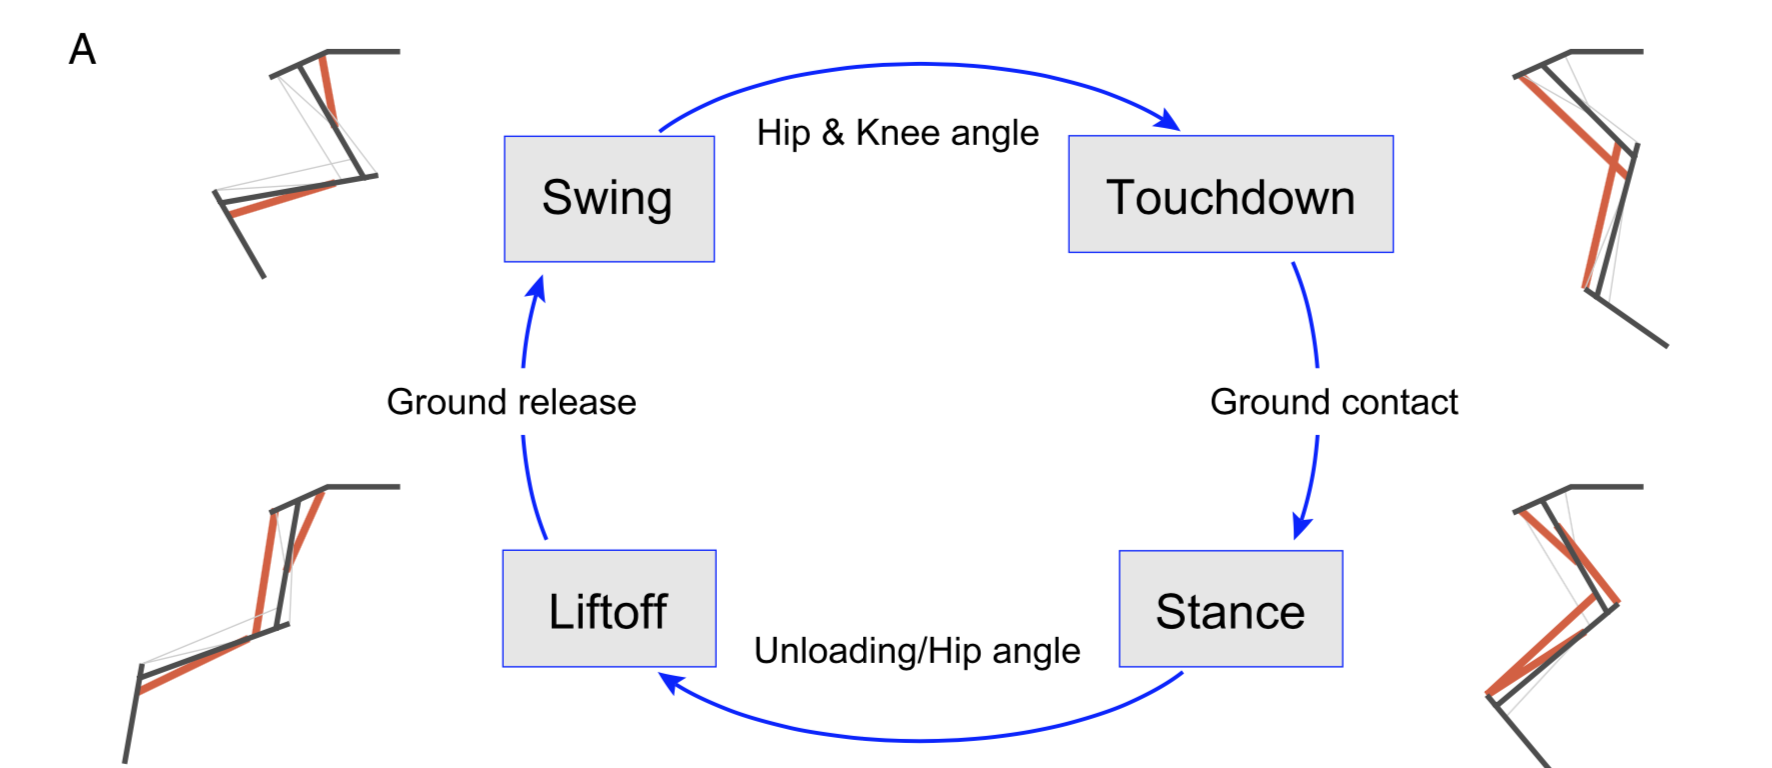
\includegraphics[width=\textwidth]{figures/ekeberg_gait}
  \caption[ekeberg gait phases]{Four stages of gait cycle as defined
    by [1] }
  \label{fig:ekeberg_gait}
\end{figure}

\begin{itemize}
\item SWING
\item TOUCH-DOWN
\item STANCE
\item LIFT-OFF
\end{itemize}

A predefined set of muscle activations make the transition between
each of the above mentioned states.  The timing between transitions is
governed by the feedback the reflex model receives. The reflex model
receives three main feed backs.
\begin{itemize}
\item Muscle forces from each muscle in the hind limb
\item Joint angles from each each joint in the hind limb
\item Foot ground contact from the hind limb
\end{itemize}

In this model, from the feed backs mentioned above we explore the
following feed backs.

\begin{itemize}
\item Hip and Knee joint angle
\item Ankle muscle forces
\item Foot ground contact
\end{itemize}

Using the above feed backs, we define the reflex conditions for
transition between the four stages of the gait and eventually produce
stable locomotion.

During the exercises in the file \corr{reflexes.py} you need to tune
the muscle activations to obtain the phase transitions and then
eventually locomotion.

\newpage

\subsection*{Code organization}
\label{subsec:code}

\begin{itemize}
\item Path to the controller files and modules -
  \corr{Lab7::Webots::controllers::mouse}
\item \corr{musculoskeletal::MusculoSkeletalSystem.py} - Class to
  read, initialize and update muscles joint system.
\item \corr{musculoskeletal::Joint.py} - Class describing the Joints
  in the system
\item \corr{musculoskeletal::Muscle.py} - Class describing the Muscle
  model in the system
\item \corr{musculoskeletal::MuscleJoint.py} - Class describing the
  interface between muscles and joints.  Converts muscle forces to
  joint torques.
\item \corr{musculoskeletal::SystemParameters.py} - Class containing
  the access properties for system parameters.
\item \corr{mouse.py} - Main class containing the Webots controller
  file. You can implement all your code in this file. Or implement in
  an external file and then do function calls from within this file as
  per your convenience.
\item \corr{reflexes.py} - Class containing the reflex model.  This is
  where you need to tune the muscle activations
\item \corr{muscle\_visualization.py} - Class for visualizing the
  muscles.  You do not have to edit this file.
\end{itemize}


\newpage
\section*{Running the simulation}

\subsection*{Make sure you have successfully installed Webots by
  following the instructions outlined in Lab 6}

\subsection*{Complete the tutorial and practice examples of Webots as
  outlined in Lab 6}

\subsection*{Open the cmc\_mouse.wbt file in Webots. This should
  launch the mouse model in simulation world}

\subsection*{Compiling the physics plugin to make the mouse fixed}

You will need to compile the physics plugin in Webots that allows you
to fix the mouse in air. To do this follow the steps below,

\begin{itemize}
\item Navigate to the WorldInfo in the SceneTree
\item Expand the WorldInfo Node
\item Click on the physics entity
\item A small dialog should now appear below. Now choose Edit option
  in the dialog
\item This should open a text editor window
\item Now go to Build in the main menu and choose the option
  \textit{Clean}
\item Next in the same Build menu choose the option \textit{Build}
\item This should now compile and build the fix\_mouse physics plugin.
\end{itemize}

\subsection*{Running the simulation}
Now when you run the simulation, the hind limb legs should drop while
the mouse is fixed in air. At this point you can now start to tune
your reflex model.

\subsection*{Explore the main mouse controller file
  \corr{mouse.py} and understand how the controller is set-up}
\corr{mouse.py} steps the Webots simulation at set time step of
1ms. During each step, the controller calls the pre-initialized
\corr{musculoskeletal::MusculoSkeletalSystem.py} class and
updates. This update computes the muscle forces based on the joint
angles and muscle activations received from the reflex controller
class.  Then the joint torques from the update are applied to Webots
rotational motors. This cycle is repeated every time step.

\section*{Questions}
\subsection*{7a. Now that you have the simulation model set-up, the
  first goal is to tune the muscle activations for each of the four
  gait stages/phases mentioned in the reflex model description
  \ref{fig:ekeberg_gait}. To do so, in \corr{reflexes.py::step} start
  un-commenting each phase and then tune the muscle activation
  constants (Kx) ranging between [0-1] to make the hind limbs move to
  the particular posture of the phase. Once you tune a particular
  posture comment the same lines in \corr{reflexes.py::step} and
  repeat the process for other phases. At this point it is not
  necessary to be very precise with the parameter tuning.  Report the
  parameters used and show a picture of the model for each of the four
  phases}

\subsection*{7b. Once you have all the phases tuned individually,
  uncomment the left and right leg state transition lines in
  \corr{reflexes.py::step}.  (Note : Make sure to comment the
  individual phase tuning lines in \corr{reflexes.py::step}). You
  should now observe a walk like gait if everything goes well. Global
  position of the hind feet is saved in the
  \corr{controllers::mouse::Results} by default after you revert the
  simulation. Plot the trajectory of both the hind feet and explain if
  the behavior is a limit cycle or not. You may use the function
  \corr{controllers::mouse::Results::load\_data.py} to read the saved
  data.}

\newpage

\section*{REFERENCES}
\label{sec:references}

1. \textit{Computer Simulation of Stepping in the Hind Legs of the
  Cat: An Examination of Mechanisms Regulating the Stance-to-Swing
  Transition} : Orjan Ekeberg and Keir Pearson. Journal of
Neurophysiology 2005 94:6, 4256-4268
\href{https://www.physiology.org/doi/abs/10.1152/jn.00065.2005}{\corr{download
    link}}


\newpage
\section*{APPENDIX}
\label{sec:appendix}


\subsection*{Muscle Attachment Simplification}
\label{sec:muscle-attachment}

In Lab 5 you have explored the role of muscle attachment points across
a given joint. From the results it was also clear that the role of
muscle attachment can be analytically pre-computed. In this model, an
analytical approach is used to pre-compute the change in muscle length
and muscle moment arm for a given joint angle.

\subsubsection*{Moment Arm}
\label{sec:moment-arm}

The force produced by the muscles needs to be transformed into a
moment before being applied to the joints.

\begin{equation}
  \label{eq:moment_arm}
  \tau = M_{\theta \rightarrow \tau }(\theta, \theta_{max}) \times F_{mtu}
\end{equation}

Where,
\begin{itemize}
\item $\tau$ : Moment/Torque produced by the muscle [$N-m$]
\item $M_{\theta \rightarrow \tau }(\theta, \theta_{max})$ : Moment
  Arm as a function of $\theta$ and $\theta_{max}$[$m$]
\item $\theta_{max}$ : Joint angle at which maximum moment is applied
  [$rad$]
\item $F_{mtu}$ : Force produced by muscle tendon unit [$N$]
\end{itemize}

Equation \ref{eq:moment_arm} shows the transfer of muscle force to
joint torque.  In order to simplify the model and the complexities
that arise due to the muscle moment arm change, we simplify the
equation \ref{eq:moment_arm} by avoiding the joint torque as function
of joint Angle $\theta$. Equation \ref{eq:moment_arm_simple} shows the
simplified equation where moment arm is now a constant maximum value
$r_0$.

\begin{equation}
  \label{eq:r_0}
  M_{\theta \rightarrow \tau}(\theta_{max}) = r_0
\end{equation}

\begin{equation}
  \label{eq:moment_arm_simple}
  \tau = r_0 \times F_{mtu}
\end{equation}

Where,
\begin{itemize}
\item $r_0$ : Maximum muscle moment arm [$m$]
\end{itemize}

\subsubsection*{Muscle Length}
\label{sec:muscle-length}

As with the moment arm, change in muscle length can be also be defined
as a function of joint angle. Equation \ref{eq:muscle_length} shows
the how the change in muscle length can be computed as a function of
joint angle.

\begin{equation}
  \label{eq:muscle_length}
  \triangle l_{mtu} = pennation \times \int^{\theta}_{\theta_{ref}} M_{\theta \rightarrow \tau}(\theta_{max})
\end{equation}

Substituting \ref{eq:r_0} in \ref{eq:muscle_length} and solving the
integral, we obtain the equation for change in muscle length as a
function of joint angle. The equation is shown in
\ref{eq:muscle_length_full}

\begin{equation}
  \label{eq:muscle_length_full}
  \triangle l_{mtu} = pennation \times r_0 \times (\theta - \theta_{ref})
\end{equation}

Where,
\begin{itemize}
\item $\triangle l_{mtu}$ : Change in muscle length [$m$]
\item $pennation$ : Angle of muscle fibers in the muscle [$rad$]
\item $r_0$ : Maximum muscle moment arm [$m$]
\item $\theta_{ref}$ : Joint angle at which muscle is at its resting
  length [$rad$]
\end{itemize}

Finally the muscle length is computed as,

\begin{equation}
  \label{eq:muscle_tendon_length}
  l_{mtu} = l_{opt} + l_{slack} + \triangle l_{mtu}
\end{equation}

Where,
\begin{itemize}
\item $l_{mtu}$ : Muscle Tendon Unit length [$m$]
\item $l_{opt}$ : Muscle optimal fiber length [$m$]
\item $l_{slack}$ : Muscle tendon slack length [$m$]
\end{itemize}



\end{document}

%%% Local Variables:
%%% mode: latex
%%% TeX-master: t
%%% End:
